\section{Mathematical Modeling}
\subsection{Derivation of the Voltage Conversion Equation}
\subsubsection*{Energy Stored During the ON Phase}
During the ON phase, the current in the primary winding increases linearly due to the applied input voltage ($V_{in}$). The rate of change of current is given by:
\[
\frac{dI_p}{dt} = \frac{V_{in}}{L_p}
\]
where:
\begin{itemize}
    \item $I_p$: Primary winding current.
    \item $L_p$: Inductance of the primary winding.
\end{itemize}

The total energy stored in the primary winding during the ON phase is:
\[
E_{stored} = \frac{1}{2} L_p I_p^2
\]

The peak primary current ($I_p$) at the end of the ON phase can be expressed as:
\[
I_p = \frac{V_{in} \cdot D \cdot T_s}{L_p}
\]
where:
\begin{itemize}
    \item $D$: Duty cycle (fraction of time the switch is ON).
    \item $T_s$: Switching period ($T_s = 1/f_s$, where $f_s$ is the switching frequency).
\end{itemize}

Substituting $I_p$ into the energy equation:
\[
E_{stored} = \frac{1}{2} L_p \left(\frac{V_{in} \cdot D \cdot T_s}{L_p}\right)^2
\]
\[
E_{stored} = \frac{1}{2} \cdot \frac{(V_{in} \cdot D \cdot T_s)^2}{L_p}
\]

\subsubsection*{Energy Transferred During the OFF Phase}
During the OFF phase, the energy stored in the transformer is transferred to the load. The output power ($P_{out}$) is related to the energy transferred per switching cycle:
\[
P_{out} = \frac{E_{transferred}}{T_s}
\]

Since the energy stored in the transformer is equal to the energy transferred to the load in steady-state:
\[
E_{transferred} = E_{stored}
\]

Thus:
\[
P_{out} = \frac{E_{stored}}{T_s}
\]

Substitute $E_{stored}$:
\[
P_{out} = \frac{1}{2} \cdot \frac{(V_{in} \cdot D \cdot T_s)^2}{L_p \cdot T_s}
\]
\[
P_{out} = \frac{1}{2} \cdot \frac{V_{in}^2 \cdot D^2 \cdot T_s}{L_p}
\]

\subsubsection*{Relating Output Voltage to Input Voltage}
The output power ($P_{out}$) is also given by:
\[
P_{out} = V_{out} \cdot I_{out}
\]

Assuming the output current ($I_{out}$) is constant and related to the duty cycle, we can express the relationship between the input and output voltages using the transformer turns ratio ($N_s/N_p$).

From the transformer equations:
\[
\frac{V_{out}}{V_{in}} = \frac{N_s}{N_p} \cdot D
\]

Rearranging:
\[
V_{out} = \frac{N_s}{N_p} \cdot D \cdot V_{in}
\]
\subsection{Power Stage Calculation Formulas}
\subsubsection*{1. Duty Cycle ($D$)}
$$
D = \frac{\frac{V_{out}}{V_{in}}}{\frac{N_s}{N_p} + \frac{V_{out}}{V_{in}}}
$$
The duty cycle determines the fraction of time the switch is ON during a switching cycle. It depends on the input/output voltages and the transformer turns ratio.

\subsubsection*{2. Load Resistance ($R_{load}$)}
$$
R_{load} = \frac{V_{out}}{I_{out}}
$$
The load resistance is calculated from the output voltage and current. It represents the effective resistance seen by the converter.

\subsubsection*{3. Output Current ($I_{out}$)}
$$
I_{out} = \frac{P_{out}}{V_{out}}
$$
The output current is derived from the output power and voltage. It indicates the current supplied to the load.

\subsubsection*{4. Ripple Current ($\Delta I_L$)}
$$
\Delta I_L = 0.3 \cdot I_{in}, \quad I_{in} = \frac{P_{out}}{V_{in}}
$$
The ripple current is typically chosen as 30\% of the average input current. It ensures stable operation in Continuous Conduction Mode (CCM).

\subsubsection*{5. Ripple Voltage ($\Delta V_{out}$)}
$$
\Delta V_{out} = 0.01 \cdot V_{out}
$$
The ripple voltage is assumed to be 1\% of the output voltage. It represents the allowable voltage fluctuation at the output.

\subsubsection*{6. Magnetizing Inductance ($L_m$)}
$$
L_m = \frac{V_{in} \cdot D}{f_{sw} \cdot \Delta I_L}
$$
The magnetizing inductance determines the energy stored in the transformer during the ON time of the switch.

\subsubsection*{7. Primary Inductance ($L_p$)}
$$
L_p = L_m
$$
The primary inductance is equal to the magnetizing inductance.

\subsubsection*{8. Secondary Inductance ($L_s$)}
$$
L_s = L_p \cdot \left(\frac{N_s}{N_p}\right)^2
$$
The secondary inductance is scaled by the square of the transformer turns ratio.

\subsubsection*{9. Magnetizing Inductor Ripple Current}
- Maximum Current:
$$
I_{max} = I_{in} + \frac{\Delta I_L}{2}
$$
- Minimum Current:
$$
I_{min} = I_{in} - \frac{\Delta I_L}{2}
$$
- Average Current:
$$
I_{avg} = I_{in}
$$
These values represent the peak, minimum, and average currents in the magnetizing inductor.
\newpage
\subsection{CCM and DCM Waveform}
\begin{multicols}{2}  % Start two-column layout
    % First column: image 1
    \noindent
    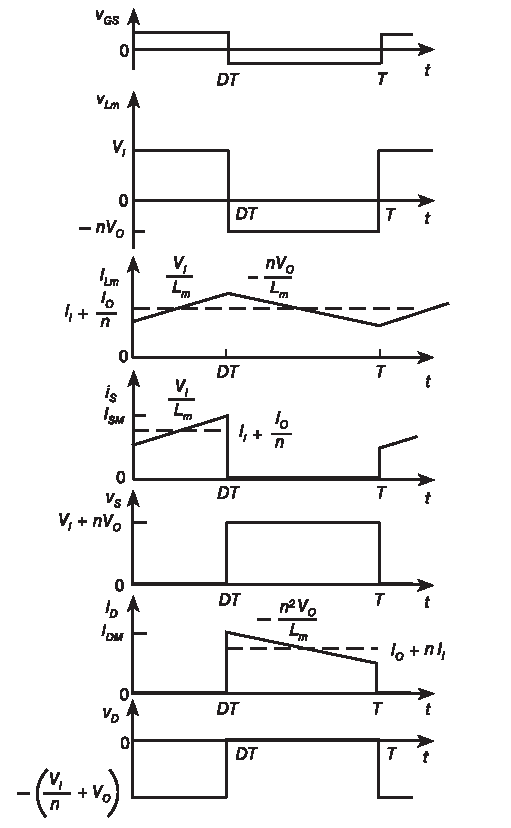
\includegraphics[width=1.07\linewidth]{Pictures/pics/7.pdf}
    \captionof{figure}{\textcolor{blue}{\textit{\footnotesize Idealized current and voltage waveforms in the PWM inverting flyback converter for CCM.}}}
    \hfill
    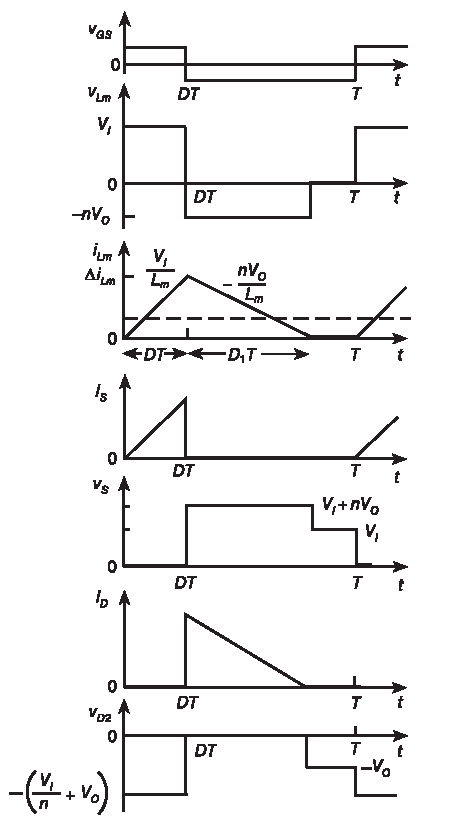
\includegraphics[width=1\linewidth]{Pictures/pics/8.pdf}
    \captionof{figure}{\textcolor{blue}{\textit{\footnotesize Idealized current and voltage waveforms in the PWM flyback converter for DCM}}}
\end{multicols}